\documentclass[conference]{IEEEtran}
\IEEEoverridecommandlockouts
% The preceding line is only needed to identify funding in the first footnote. If that is unneeded, please comment it out.
\usepackage{cite}
\usepackage{amsmath,amssymb,amsfonts}
\usepackage{algorithmic}
\usepackage{graphicx}
\usepackage{textcomp}
\usepackage{xcolor}
\def\BibTeX{{\rm B\kern-.05em{\sc i\kern-.025em b}\kern-.08em
    T\kern-.1667em\lower.7ex\hbox{E}\kern-.125emX}}
\begin{document}

\title{An End-to-End solution to Autonomous Driving based on Xilinx FPGA\\
{\footnotesize \textsuperscript{*}Note: Sub-titles are not captured in Xplore and
should not be used}
\thanks{Identify applicable funding agency here. If none, delete this.}
}

\author{\IEEEauthorblockN{1\textsuperscript{st} Tianze Wu}
\IEEEauthorblockA{\textit{Xilinx} \\
\textit{ICT}\\
Shanghai, China \\
1369130123@qq.com}
\and
\IEEEauthorblockN{2\textsuperscript{nd} Weiyi Liu}
\IEEEauthorblockA{\textit{Xilinx} \\
\textit{Shanghai JiaoTong University}\\
Shanghai, China \\
liuweiyi@sjtu.edu.cn}
\and
\IEEEauthorblockN{3\textsuperscript{rd} Given Name Surname}
\IEEEauthorblockA{\textit{Xilinx} \\
\textit{Xidian University}\\
Shanghai, China \\
yongweijin@outlook.com}
}

\maketitle

\begin{abstract}
Nowadays, the autonomous driving topic is very hot, many people are trying to provide a solution to this problem. This time we build our own auto-driving car based on Xilinx Pynq-Z2, it provides an end-to-end solution to autonomous driving and it uses the power of DPU to accelerate the computing.
\end{abstract}

\begin{IEEEkeywords}
Autonomous Driving, Machine Learning, PYNQ-Z2, Field programmable gate arrays, Computer Vision
\end{IEEEkeywords}

\section{Introduction}
Autonomous Driving is getting more and more attention recently. The main problem to be solved in this area is how to meet the need of real-time computing. 
Though we now have many customed chips like GPU and TPU for machine learning acceleration, they are not able to 
provide both high performance and low power consumpation. Also they are not flexible enough to adapt to different scenes. 
To meet these requests, FPGA is a good solution since it can provide high performance and low power consumpation, most importantly it's easy to custom accelerator for 
specified algorithms.

This time we build our own auto-driving car based on Xilinx Pynq-Z2, it provides an end-to-end solution to autonomous driving and it uses the power of DPU to accelerate the computing. 

We find that in previous FPT competitions, many competitors use traditional computer vision methods or machine learning methods to detect objects and then make decisions based on the results. Our solution is quite different with theirs since we use a simple CNN model as our AI network and feed the model with pictures taken by the camera in the car and the model returns the control orders.
The platform we use is Xilinx’s Pynq-Z2 board, there is a DPU IP in its FPGA, with DPU’s help, we can accelerate the inference process of the model and make it possible to run AI inference task in limited resource platform like Pynq-Z2.

The rest of this paper is organized as follows. Section II describes the overview of our hardware structure and development environment. Section III presents the software architecture and details of methods we are going to use for the competition. Finally, the paper mentions the current progress and makes an conclusion.

\section{Overview of our car}

\subsection{Hardware structure}

The Fig.~\ref{co} is our robot car's photograph. Its body is made of acrylic board. There is one Pynq-Z2 board as the controller, it has a DPU IP for acceleration, the sensors we use now contains a camera only. The car has one capstan motor and one electric steering engine. Two rear wheels provide power while two front wheels provide steering capacity. We use two batteries to provide power, one for the Pynq board and one for the motors.

\begin{figure}[htbp]
%\centerline{\includegraphics{fig1.png}}
\caption{Car overview.}
\label{co}
\end{figure}

\subsection{Development environment}

The operating system we use in the car is created by PetaLinux, it has opencv and dpu support. We control the motors by directly writing values to physical memory address of FPGA, the drivers are implemented in FPGA. Most of our AI inference computing tasks are run by DPU, the tasks which DPU doesn't support are run by arm core embedded in Pynq-Z2. The driving decisions are made by AI model while the central controller is run in arm core.  

We provide two language implementations for collect-data module, you can collect data for training in c++ or python environment. The c++ version is more commonly used while the python version has a good support in Pynq-Z2. The auto-run module is implemented in c++ since the DNNDK-v3.0 version has only APIs for c++ language.

\section{Software Implementation and algorithms}

In most tasks, our solution can completely rely on machine learning methods, such as left-side driving, obstacle avoidance and crossroad driving. When it comes to other scenes, we use traditional computer vision algorithms and state machine to help us finish the task. The car only uses a camera as the sensor now, we may add some more sensors if a camera is not enough.

\subsection{Software architecture}\label{AA}

In our design, we aim to make the platform be easy to use and expand. There are three main modules in our system.

\begin{itemize}
\item The first part is Data Collect module. It needs human to control the car to finish some driving tasks. The program will record the images taken and real-time commands during the process. These data will be used as training data.
\item The second part is PC Host module. Since our edge devices cannot provide huge compution power, we will use more powerful devices like normal computers to do the machine learning job. You can use any hardware you like to do the training and then use DNNDK provided by Xilinx to do some optimizations. DNNDK kit can do pruning, quantization, compilation and optimization to the trained model. After this step, we will have DPU kernels that can help us accelerate inference process in the car.
\item The third part is Autonomous Driving module, it acts like the first module but the human controller of the car is replaced by machine learning network.
\end{itemize}

Since these three parts are separated, so it's easy to modify one module without affecting others. It will be easy to build a different neural network or use different hardware devices. We are also working on an virtual simulator for our platform, once it is finished you can train or evaluate the model based on virtual environment. This can help people build or test their model structure efficiently.
\begin{figure}[htbp]
\centerline{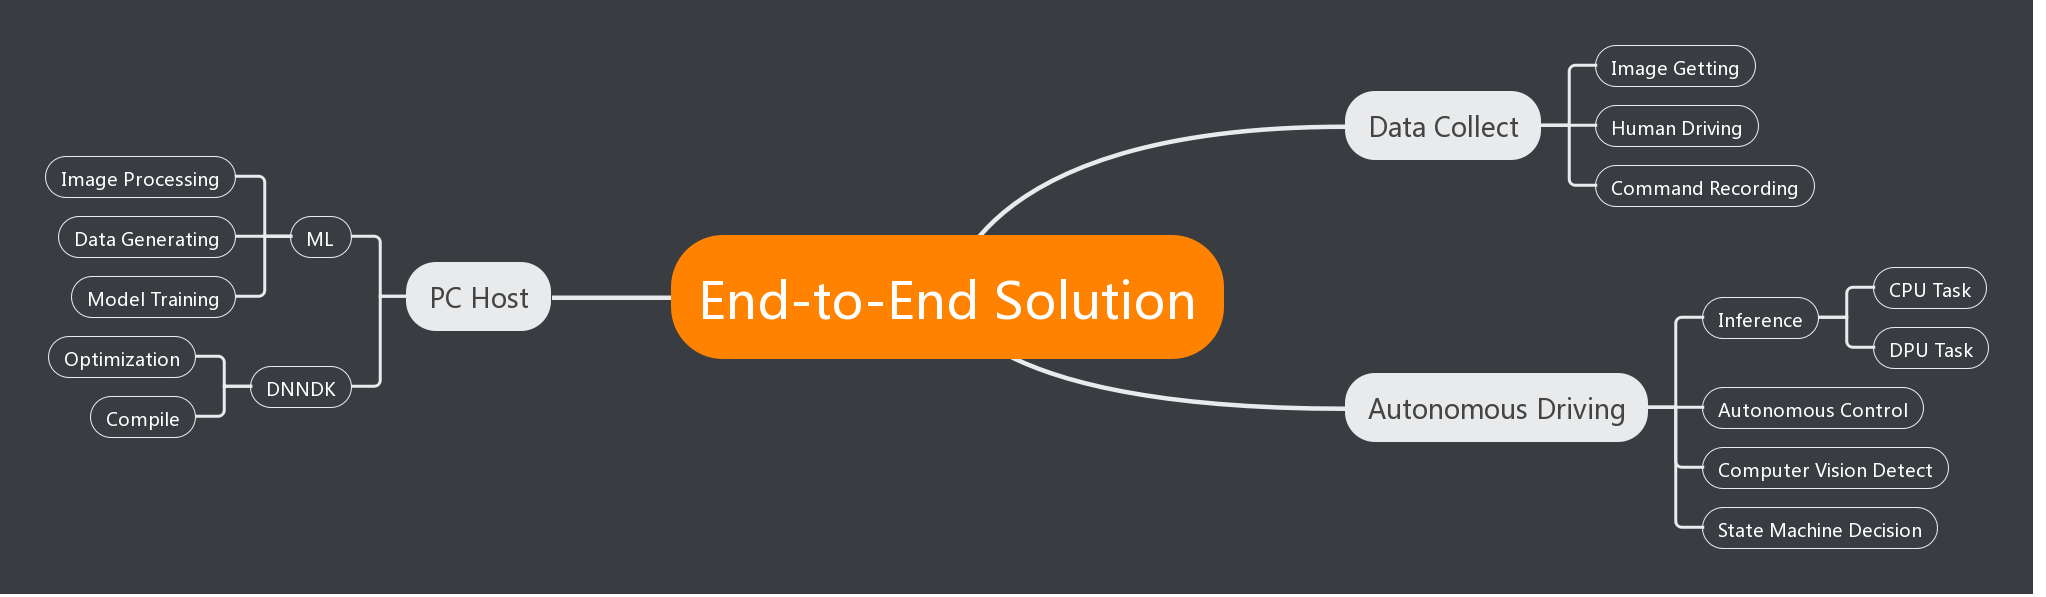
\includegraphics[width=0.5\textwidth]{software-architecture.jpg}}
\caption{Software Architecture}
\label{sa}
\end{figure}

\subsection{Work flow}

Fig.~\ref{wf} shows the control flow of our autonomous driving. The car can run in two mode, one is that the car will be in total control of machine learning methods, the other means that the traditional computer vision methods will be used when the car runs into the situation in which neural network is not able to handle.

The whole system will have one worker for running computer vision methods like objects recognition and one worker for taking photos. The number of the workers for machine learning tasks can be specified since it's meaningful to run parallel tasks in DPU.

\begin{figure}[htbp]
\centerline{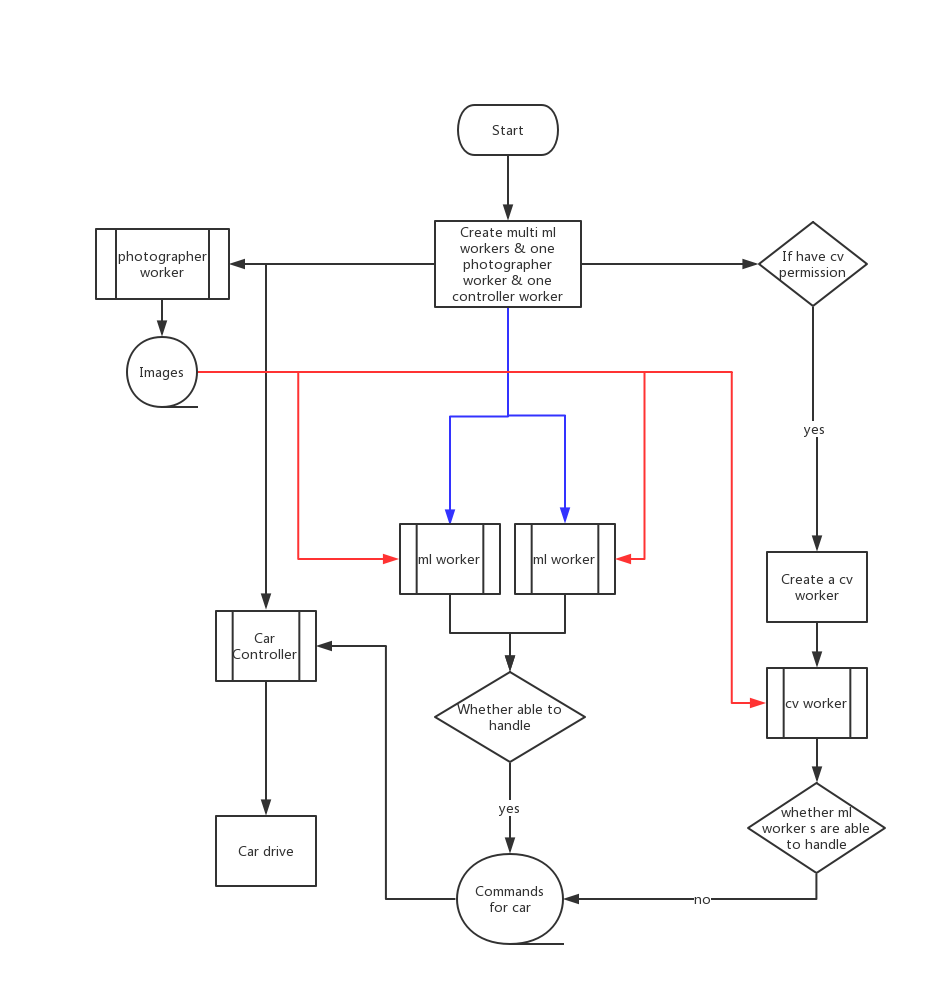
\includegraphics[width=0.5\textwidth]{workFlow.jpg}}
\caption{Work Flow}
\label{wf}
\end{figure}

\subsection{AI model}

The network we use is a simple end-to-end model. Since the DNNDK kit doesn't support some AI functions, we adapt our model to DNNDK. The structure of the model is shown in Fig.~\ref{ms}.

\begin{figure}[htbp]
%\centerline{\includegraphics{fig1.png}}
\caption{Model Structure.}
\label{ms}
\end{figure}

The main part of the model is CNN layers, they can extract features from the images taken by the car's front camera. Some fully connected layers follow the CNN layers, they can finally extract the command information needed for auto-driving. The activation function we use is Relu because it works well and can be accelerated by DPU. The last layer is a Softmax layer, it can provide classification and normalization functions for the model.  

Although the current model is not the perfect one and it cannot be accelerated by DPU totally, it's easy to make changes and optimizations to the model. With the development of DNNDK, more portion of the model can be accelerated and the whole system can be more efficient and powerful.

\subsection{Algorithms}
\begin{itemize}
\item Crossroad control. Since the AI model cannot handle the situation when the car meets a crossroad. We will help the car decide which direction to take according to the competition's request. The car will use neural network or cv algorithms to recognize all the scenes that need it to make a choice, for example the crossroad. After the car meets these scenes, first the main controller will tell the car which direction to take, then the car will use predefined control commands to drive through the crossroad. When this progress is finished, the AI model will retake the control of the car.
\item Image process. Although our solution is end-to-end, the training data needs to be processed. Now we just do the normalization to the input images, later we will try some more according to the evaluation of the model's performance.
\item Obstacle avoidance. For obstacle avoidance, traditional methods will first recognize the objects from the image and then use the state machine functions to make decisions. Our solution is quite different from it, we will add the obstacle avoidance scenes to the step of collecting training data. As a result, when the training step is finished, the AI model can avoid the obstacle automatically.
\end{itemize}

\section{Development status}

Until now, we have built the whole system, the AI model works well in simple scenes. We are busy implementing the cv functions and optimizing the hardware structure of the car. Later we will try to make some improvements to the model and do some tests and modifications according to the competition's rules. If possible, we will build a simulator to generate training data and evaluate the system. Our goal is not only winning the competition, but also building a general and easy-to-use platform for those who want to try their own ideas about auto-driving.

\section{Conclusion}

The DPU embedded in FPGA accelerates the inference progress of AI algorithms. Our team wants to use this great power to build an autonomous driving system, with the help of Xilinx's Pynq-Z2 and DNNDK, our project will provide people with a new version of end-to-end autonomous driving solution.

We will focus on the stability of the system and the cooperations between AI network and traditional methods in the next step.

\begin{table}[htbp]
\caption{Table Type Styles}
\begin{center}
\begin{tabular}{|c|c|c|c|}
\hline
\textbf{Table}&\multicolumn{3}{|c|}{\textbf{Table Column Head}} \\
\cline{2-4} 
\textbf{Head} & \textbf{\textit{Table column subhead}}& \textbf{\textit{Subhead}}& \textbf{\textit{Subhead}} \\
\hline
copy& More table copy$^{\mathrm{a}}$& &  \\
\hline
\multicolumn{4}{l}{$^{\mathrm{a}}$Sample of a Table footnote.}
\end{tabular}
\label{tab1}
\end{center}
\end{table}

\section*{Acknowledgment}

The preferred spelling of the word ``acknowledgment'' in America is without 
an ``e'' after the ``g''. Avoid the stilted expression ``one of us (R. B. 
G.) thanks $\ldots$''. Instead, try ``R. B. G. thanks$\ldots$''. Put sponsor 
acknowledgments in the unnumbered footnote on the first page.

\section*{References}

Please number citations consecutively within brackets \cite{b1}. The 
sentence punctuation follows the bracket \cite{b2}. Refer simply to the reference 
number, as in \cite{b3}---do not use ``Ref. \cite{b3}'' or ``reference \cite{b3}'' except at 
the beginning of a sentence: ``Reference \cite{b3} was the first $\ldots$''

Number footnotes separately in superscripts. Place the actual footnote at 
the bottom of the column in which it was cited. Do not put footnotes in the 
abstract or reference list. Use letters for table footnotes.

Unless there are six authors or more give all authors' names; do not use 
``et al.''. Papers that have not been published, even if they have been 
submitted for publication, should be cited as ``unpublished'' \cite{b4}. Papers 
that have been accepted for publication should be cited as ``in press'' \cite{b5}. 
Capitalize only the first word in a paper title, except for proper nouns and 
element symbols.

For papers published in translation journals, please give the English 
citation first, followed by the original foreign-language citation \cite{b6}.

\begin{thebibliography}{00}
\bibitem{b1} G. Eason, B. Noble, and I. N. Sneddon, ``On certain integrals of Lipschitz-Hankel type involving products of Bessel functions,'' Phil. Trans. Roy. Soc. London, vol. A247, pp. 529--551, April 1955.
\bibitem{b2} J. Clerk Maxwell, A Treatise on Electricity and Magnetism, 3rd ed., vol. 2. Oxford: Clarendon, 1892, pp.68--73.
\bibitem{b3} I. S. Jacobs and C. P. Bean, ``Fine particles, thin films and exchange anisotropy,'' in Magnetism, vol. III, G. T. Rado and H. Suhl, Eds. New York: Academic, 1963, pp. 271--350.
\bibitem{b4} K. Elissa, ``Title of paper if known,'' unpublished.
\bibitem{b5} R. Nicole, ``Title of paper with only first word capitalized,'' J. Name Stand. Abbrev., in press.
\bibitem{b6} Y. Yorozu, M. Hirano, K. Oka, and Y. Tagawa, ``Electron spectroscopy studies on magneto-optical media and plastic substrate interface,'' IEEE Transl. J. Magn. Japan, vol. 2, pp. 740--741, August 1987 [Digests 9th Annual Conf. Magnetics Japan, p. 301, 1982].
\bibitem{b7} M. Young, The Technical Writer's Handbook. Mill Valley, CA: University Science, 1989.
\end{thebibliography}
\vspace{12pt}

\end{document}
